\chapter{Introdução a Grafos}

Grafos são uma das abstrações mais versáteis da Computação. 
Sempre que precisamos modelar entidades e suas relações --- pessoas e amizades, cidades e estradas, páginas e links, tarefas e dependências --- estamos, essencialmente, lidando com grafos. 
Nesta aula, apresentaremos a ideia central, os conceitos básicos, os principais tipos, algumas propriedades elementares, o problema clássico das pontes de Königsberg, aplicações, e as representações mais usadas em código (matriz e lista de adjacência).

\section{O que são grafos}

Um \textbf{grafo} é formado por um conjunto de \textbf{vértices} (ou \emph{nós}) e um conjunto de \textbf{arestas} que conectam pares de vértices. 
Intuitivamente, vértices representam objetos e arestas representam relações entre esses objetos.

Exemplos cotidianos incluem:
\begin{itemize}
  \item \textbf{Rede social:} pessoas são vértices; amizades são arestas.
  \item \textbf{Mapa:} cidades são vértices; estradas são arestas.
  \item \textbf{Dependências:} tarefas são vértices; uma aresta indica que uma tarefa depende de outra.
\end{itemize}

\section{Conceitos fundamentais}

\begin{itemize}
  \item \textbf{Vértice (nó):} entidade básica que queremos modelar.
  \item \textbf{Aresta (ligação):} relação entre dois vértices.
  \item \textbf{Grau:} número de arestas incidentes a um vértice (em dígrafos, distinguimos \emph{grau de entrada} e \emph{grau de saída}).
  \item \textbf{Caminho:} sequência de vértices conectados por arestas.
  \item \textbf{Ciclo:} caminho que começa e termina no mesmo vértice.
  \item \textbf{Conectividade:} dois vértices estão conectados se existe um caminho entre eles; um grafo é \emph{conexo} se qualquer vértice alcança qualquer outro.
  \item \textbf{Componente conexa:} subgrafo conexo maximal.
\end{itemize}

\section{Tipos de grafos}

Dependendo da natureza da relação, usamos variantes de grafos:

\begin{center}
\renewcommand{\arraystretch}{1.3}
\begin{tabular}{@{}p{2.8cm} p{6cm} p{5cm}@{}}
\toprule
\textbf{Tipo} & \textbf{Descrição} & \textbf{Exemplo prático} \\
\midrule
\textbf{Não direcionado} & Arestas sem orientação (relação bidirecional). & Amizade em redes sociais. \\
\textbf{Direcionado (dígrafo)} & Arestas orientadas ($u \to v$). & Seguidores no Twitter, fluxo de dados. \\
\textbf{Ponderado} & Arestas com pesos (custo, tempo, distância). & Rotas de transporte. \\
\textbf{Multigrafo} & Arestas paralelas entre o mesmo par de vértices. & Linhas distintas entre duas cidades. \\
\textbf{Com laços} & Aresta que liga um vértice a si próprio. & Dependência recursiva. \\
\bottomrule
\end{tabular}
\end{center}


\subsection*{Diagramas ilustrativos}

% estilos locais
\newcommand{\tikzstyleset}{
\tikzset{
  vertex/.style={draw,circle,minimum size=8mm,inner sep=0pt},
  edgeu/.style={-,thick},
  edged/.style={-{Latex},thick},
  lbl/.style={font=\small,fill=white,inner sep=1pt}
}
}

\begin{center}
\begin{minipage}{0.9\textwidth}
\centering
\textbf{Grafo não direcionado}\\[4pt]
\begin{tikzpicture}[node distance=22mm]
\tikzstyleset
  \node[vertex] (A) {A};
  \node[vertex, right=of A] (B) {B};
  \node[vertex, below=of $(A)!0.5!(B)$] (C) {C};
  \draw[edgeu] (A)--(B);
  \draw[edgeu] (B)--(C);
  \draw[edgeu] (C)--(A);
\end{tikzpicture}\\[2pt]
\emph{Arestas sem orientação.}
\end{minipage}

\bigskip
\begin{minipage}{0.9\textwidth}
\centering
\textbf{Grafo direcionado (dígrafo)}\\[4pt]
\begin{tikzpicture}[node distance=24mm]
\tikzstyleset
  \node[vertex] (A) {A};
  \node[vertex, right=of A] (B) {B};
  \node[vertex, below=of $(A)!0.5!(B)$] (C) {C};
  \draw[edged] (A)--(B);
  \draw[edged] (B)--(C);
  \draw[edged] (C)--(A);
\end{tikzpicture}\\[2pt]
\emph{Arestas com sentido ($u\to v$).}
\end{minipage}

\bigskip
\begin{minipage}{0.9\textwidth}
\centering
\textbf{Grafo ponderado}\\[4pt]
\begin{tikzpicture}[node distance=28mm]
\tikzstyleset
  \node[vertex] (A) {A};
  \node[vertex, right=of A] (B) {B};
  \node[vertex, below=of $(A)!0.5!(B)$] (C) {C};
  \draw[edgeu] (A)--(B) node[midway,above,lbl]{10};
  \draw[edgeu] (A)--(C) node[midway,left,lbl]{5};
  \draw[edgeu] (B)--(C) node[midway,right,lbl]{7};
\end{tikzpicture}\\[2pt]
\emph{Cada aresta carrega um custo ou distância.}
\end{minipage}

\bigskip
\begin{minipage}{0.9\textwidth}
\centering
\textbf{Multigrafo (arestas paralelas)}\\[4pt]
\begin{tikzpicture}[node distance=40mm]
\tikzstyleset
  \node[vertex] (A) {A};
  \node[vertex, right=of A] (B) {B};
  \draw[edgeu, bend left=20]  (A) to node[above,lbl]{L1} (B);
  \draw[edgeu, bend right=20] (A) to node[below,lbl]{L2} (B);
\end{tikzpicture}\\[2pt]
\emph{Mais de uma aresta entre o mesmo par de vértices.}
\end{minipage}

\bigskip
\begin{minipage}{0.9\textwidth}
\centering
\textbf{Grafo com laço}\\[4pt]
\begin{tikzpicture}[node distance=28mm]
\tikzstyleset
  \node[vertex] (D) {D};
  \node[vertex, right=of D] (E) {E};
  \draw[edged] (D)--(E);
  \path (D) edge[loop above,thick] node[lbl]{w} ();
\end{tikzpicture}\\[2pt]
\emph{Aresta que sai e retorna ao mesmo vértice.}
\end{minipage}
\end{center}


\section{Propriedades básicas}

\begin{itemize}
  \item \textbf{Ordem} de um grafo: número de vértices ($|V|$).
  \item \textbf{Tamanho} de um grafo: número de arestas ($|E|$).
  \item \textbf{Soma dos graus (não direcionado):} $\sum_{v\in V}\deg(v)=2|E|$.
  \item \textbf{Em dígrafos:} $\sum \deg^+(v)=\sum \deg^-(v)=|E|$.
  \item \textbf{Limite superior de arestas (sem laços):}
  \begin{itemize}
    \item \emph{Grafo não direcionado simples:} $|E|_{\max}=\dfrac{|V|(|V|-1)}{2}$.
    \item \emph{Grafo direcionado (dígrafo) simples:} $|E|_{\max}=|V|(|V|-1)$.
  \end{itemize}
  \item \textbf{Limite inferior de arestas em grafos conexos.}
\begin{itemize}
  \item \emph{Grfao não direcionado simples:} se o grafo é conexo, então
  \[
    |E| \,\ge\, |V|-1,
  \]
\end{itemize}
\end{itemize}

Essas relações ajudam a checar consistência e servem de base para algoritmos (por exemplo, muitos percorrem vizinhos de um vértice, logo custos dependem do grau).

\section{O problema das pontes de Königsberg}

Em 1736, Euler modelou o problema de atravessar todas as pontes da cidade de Königsberg sem repetir nenhuma. 
Abstraindo regiões como vértices e pontes como arestas, a pergunta torna-se: \emph{existe um caminho que use cada aresta exatamente uma vez?} (caminho euleriano).

\begin{figure}[h]
\centering
\includegraphics[width=0.4\textwidth]{konigsberg-bridges.png}
\caption{As 7 pontos de Konigsberg.}
\label{fig:konigsberg}
\end{figure}


Euler mostrou que para que exista um caminho (euleriano), o grafo deve ser conexo e ter exatamente dois vértices de grau ímpar. 
Essa condição aparece porque, ao percorrer as arestas, todo vértice intermediário é visitado um número par de vezes: a cada vez que o caminho entra por uma aresta, ele precisa sair por outra, e assim o número total de arestas incidentes a esses vértices é par. 
Já os vértices inicial e final se comportam de modo diferente: no vértice de partida há uma saída a mais que entrada, e no vértice de chegada há uma entrada a mais que saída, o que faz com que ambos tenham grau ímpar. 
Se houvesse mais de dois vértices ímpares, seria necessário começar ou terminar o percurso em mais de dois pontos, o que é impossível em um único trajeto.

\begin{center}
\begin{minipage}{0.9\textwidth}
\centering
\textbf{Abstração de Königsberg}\\[4pt]
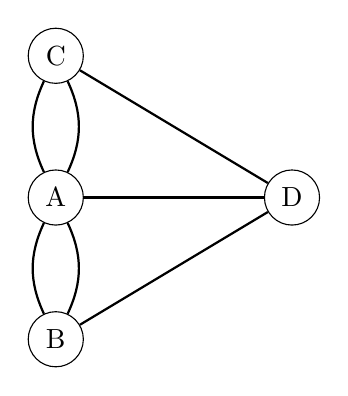
\begin{tikzpicture}[scale=1.0]
\tikzset{
  vertex/.style={draw,circle,minimum size=7mm,inner sep=0pt},
  edgeu/.style={-,thick}
}
% nós (C, A, B em coluna à esquerda; D à direita)
\node[vertex] (C) at (0,1.8) {C};
\node[vertex] (A) at (0,0)   {A};
\node[vertex] (B) at (0,-1.8){B};
\node[vertex] (D) at (3,0)   {D};

% arestas paralelas C--A
\draw[edgeu,bend left=25]  (C) to (A);
\draw[edgeu,bend right=25] (C) to (A);

% arestas paralelas A--B
\draw[edgeu,bend left=25]  (A) to (B);
\draw[edgeu,bend right=25] (A) to (B);

% arestas simples até D
\draw[edgeu] (C) -- (D);
\draw[edgeu] (A) -- (D);
\draw[edgeu] (B) -- (D);
\end{tikzpicture}\\[2pt]
\end{minipage}
\end{center}


\section{Aplicações}

Grafos aparecem em:
\begin{itemize}
  \item \textbf{Redes sociais e informação:} comunidade, influência, recomendações.
  \item \textbf{Rotas e logística:} caminhos mínimos, cobertura, árvores geradoras.
  \item \textbf{Dependências e planejamento:} ordenação topológica em DAGs.
  \item \textbf{Computação e redes:} roteamento, conectividade, tolerância a falhas.
  \item \textbf{Ciências naturais:} interações biológicas, redes metabólicas, ecologia.
\end{itemize}

\section{Tipo Abstrato de Dados (TAD) Grafos}

Nos capítulos anteriores, estudamos dois tipos de dicionário: o \textbf{dicionário simples}, baseado em tabelas de dispersão, e o \textbf{dicionário ordenado}, implementado com árvores binárias de busca.  
Essas estruturas tinham como foco associar chaves e valores de forma eficiente, seja pelo acesso direto (hash) ou pela ordenação (árvores).  
Agora, no estudo de grafos, ampliamos esse mesmo princípio de abstração para um tipo de dado mais geral, no qual os elementos não estão apenas associados a valores, mas conectados entre si.

\medskip
Assim como nos dicionários, a noção de \emph{Tipo Abstrato de Dados} (TAD) continua essencial.  
O \textbf{TAD Grafo} define um conjunto de operações que permitem manipular grafos sem se comprometer com a forma como eles são representados em memória.  
Essa separação entre o nível abstrato e o nível de implementação é fundamental porque existem várias formas possíveis de representar um grafo, cada uma com vantagens e limitações específicas.

\medskip
Do ponto de vista abstrato, um TAD Grafo deve permitir, entre outras, as seguintes operações:

\begin{itemize}
  \item \texttt{criarGrafo()}: cria um grafo vazio.
  \item \texttt{inserirVertice(v)} e \texttt{inserirAresta(u, v)}: adicionam vértices e arestas.
  \item \texttt{removerVertice(v)} e \texttt{removerAresta(u, v)}: removem elementos existentes.
  \item \texttt{adjacentes(u)}: devolve os vértices conectados a \(u\).
  \item \texttt{grau(v)}: retorna o grau de um vértice.
  \item \texttt{numVertices()} e \texttt{numArestas()}: retornam as quantidades de vértices e arestas.
\end{itemize}

Essas operações definem o comportamento lógico do grafo, isto é, o que ele deve ser capaz de fazer, sem indicar como faz.  
Dessa forma, o mesmo TAD pode ter múltiplas implementações compatíveis com os algoritmos que o utilizam — exatamente como vimos nos TADs anteriores.  
Essa abordagem é adequada porque permite estudar e comparar diferentes representações, trocando a estrutura interna sem alterar a interface pública.

\medskip
As duas representações mais tradicionais de um grafo são as seguintes:

\begin{itemize}
  \item \textbf{Matriz de adjacência:}  
  consiste em uma matriz \( |V| \times |V| \) na qual a célula \((i,j)\) indica a presença (ou o peso) de uma aresta entre os vértices \(i\) e \(j\).  
  Essa representação é simples e permite verificar a existência de uma aresta em tempo constante \(O(1)\), mas tem custo de memória proporcional ao quadrado do número de vértices:  
  \[
  \text{Espaço ocupado} = O(|V|^2)
  \]
  Mesmo que o grafo tenha poucas arestas (isto é, seja esparso), a matriz reserva espaço para todas as combinações possíveis de vértices.

  \item \textbf{Lista de adjacência:}  
  para cada vértice, mantém-se uma lista com seus vizinhos.  
  Essa estrutura ocupa espaço proporcional ao número de vértices mais o número de arestas:
  \[
  \text{Espaço ocupado} = O(|V| + |E|)
  \]
  Por isso, é muito mais eficiente para grafos grandes e esparsos, nos quais \( |E| \ll |V|^2 \).
\end{itemize}

\medskip
Em resumo, a matriz de adjacência é vantajosa em grafos \emph{densos}, com muitas conexões, pois o custo de \(O(|V|^2)\) é justificado pela rapidez de acesso.  
Já a lista de adjacência é superior em grafos \emph{esparsos}, que têm poucas arestas, economizando memória e tornando as operações de iteração sobre vizinhos mais eficientes.  

O uso do TAD Grafo nos permite abstrair essas diferenças: podemos implementar algoritmos de busca, caminhos mínimos ou árvores geradoras sem nos preocupar com o formato interno da representação.  
Se precisarmos otimizar para memória ou velocidade, basta trocar a implementação do TAD, mantendo o mesmo conjunto de operações.

\section{TAD Grafo com Matriz de Adjacência}

A seguir implementamos um grafo não-direcionado, simples e não-ponderado usando \textbf{matriz de adjacência}. 
Essa escolha facilita o teste de existência de aresta em tempo $O(1)$, ao custo de memória $O(|V|^2)$. 
As seis operações expostas aqui compõem uma interface mínima e suficiente para algoritmos clássicos (BFS, DFS, etc.).

\subsection*{Políticas de implementação}
\begin{itemize}
  \item \textbf{Índices de vértices}: inteiros de $0$ a $nV-1$.
  \item \textbf{Inserção de vértice}: cria-se um novo índice no final (incrementa $nV$).
  \item \textbf{Remoção de vértice}: \emph{compactação}: a última linha/coluna é movida para a posição do vértice removido, e $nV$ é decrementado.
  \item \textbf{Inserção/remoção de aresta}: atualizam $nE$ (\# de arestas) e mantêm a simetria da matriz.
  \item \textbf{Adjacentes(u)}: retorna, em um vetor externo, os vizinhos de $u$.
\end{itemize}

\subsection*{Cabeçalhos e estrutura}

\begin{lstlisting}
// grafo_matriz.h
#ifndef GRAFO_MATRIZ_H
#define GRAFO_MATRIZ_H

typedef struct {
    int maxV;    // capacidade máxima
    int nV;      // número atual de vértices
    int nE;      // número atual de arestas
    unsigned char *M; // matriz nV x nV (alocada com maxV x maxV)
} Graph;

// Acesso M[u][v]
#define MAT(G,u,v) ((G)->M[(u)*(G)->maxV + (v)])

// Criação/Destruição
Graph* grafo_criar(int maxV);
void    grafo_destruir(Graph *G);

// Operações pedidas (6)
int grafo_inserir_vertice(Graph *G);           // retorna índice do novo vértice ou -1
int grafo_remover_vertice(Graph *G, int v);    // retorna 0 ok, -1 erro
int grafo_inserir_aresta(Graph *G, int u, int v);   // 0 ok, -1 erro
int grafo_remover_aresta(Graph *G, int u, int v);   // 0 ok, -1 erro
int grafo_adjacentes(const Graph *G, int u, int *out, int max_out); // retorna k

// Utilitários
int grafo_num_vertices(const Graph *G);
int grafo_num_arestas(const Graph *G);

#endif // GRAFO_MATRIZ_H
\end{lstlisting}

\subsection*{Implementação}

\begin{lstlisting}
// grafo_matriz.c
#include <stdio.h>
#include <stdlib.h>
#include <string.h>
#include "grafo_matriz.h"

static int vertice_valido(const Graph *G, int v) {
    return (G && v >= 0 && v < G->nV);
}

Graph* grafo_criar(int maxV) {
    if (maxV <= 0) return NULL;
    Graph *G = (Graph*) malloc(sizeof(Graph));
    if (!G) return NULL;
    G->maxV = maxV;
    G->nV = 0;
    G->nE = 0;
    G->M = (unsigned char*) calloc((size_t)maxV * (size_t)maxV, sizeof(unsigned char));
    if (!G->M) { free(G); return NULL; }
    return G;
}

void grafo_destruir(Graph *G) {
    if (!G) return;
    free(G->M);
    free(G);
}

int grafo_num_vertices(const Graph *G) { return G ? G->nV : 0; }
int grafo_num_arestas (const Graph *G) { return G ? G->nE : 0; }

int grafo_inserir_vertice(Graph *G) {
    if (!G) return -1;
    if (G->nV == G->maxV) return -1; // capacidade esgotada
    int v = G->nV++;
    // zera linha e coluna do novo vértice dentro do bloco atual nV x nV
    for (int i = 0; i < G->nV; ++i) {
        MAT(G, v, i) = 0;
        MAT(G, i, v) = 0;
    }
    return v;
}

static int soma_linha(const Graph *G, int v) {
    int deg = 0;
    for (int j = 0; j < G->nV; ++j) deg += MAT(G, v, j);
    return deg;
}

int grafo_remover_vertice(Graph *G, int v) {
    if (!vertice_valido(G, v)) return -1;
    // remover arestas incidentes (atualiza nE)
    int deg_v = soma_linha(G, v);
    G->nE -= deg_v; // cada aresta é contada 1x na linha v (grafo não-direcionado, simetria garantida)

    int last = G->nV - 1;
    if (v != last) {
        // move a linha 'last' para 'v'
        for (int j = 0; j < G->nV; ++j) {
            MAT(G, v, j) = MAT(G, last, j);
        }
        // move a coluna 'last' para 'v'
        for (int i = 0; i < G->nV; ++i) {
            MAT(G, i, v) = MAT(G, i, last);
        }
        // zera a linha/coluna 'last' (não obrigatório, mas ajuda a depurar)
        for (int j = 0; j < G->nV; ++j) {
            MAT(G, last, j) = 0;
            MAT(G, j, last) = 0;
        }
        /* Ajuste de nE: já descontamos as arestas de v; mas ao mover 'last' para 'v',
           preservamos o número de arestas restantes pois copiamos simetricamente.
           Não há dupla contagem aqui pois as incidências de 'last' continuam existindo,
           agora rotuladas como 'v'. */
    } else {
        // apenas zera última linha/coluna
        for (int j = 0; j < G->nV; ++j) {
            MAT(G, last, j) = 0;
            MAT(G, j, last) = 0;
        }
    }
    G->nV--;
    return 0;
}

int grafo_inserir_aresta(Graph *G, int u, int v) {
    if (!vertice_valido(G, u) || !vertice_valido(G, v)) return -1;
    if (u == v) return -1; // sem laços neste TAD simples
    if (MAT(G, u, v)) return 0; // já existe; idempotente
    MAT(G, u, v) = 1;
    MAT(G, v, u) = 1;
    G->nE++;
    return 0;
}

int grafo_remover_aresta(Graph *G, int u, int v) {
    if (!vertice_valido(G, u) || !vertice_valido(G, v)) return -1;
    if (u == v) return -1;
    if (!MAT(G, u, v)) return 0; // não existe; idempotente
    MAT(G, u, v) = 0;
    MAT(G, v, u) = 0;
    G->nE--;
    return 0;
}

int grafo_adjacentes(const Graph *G, int u, int *out, int max_out) {
    if (!vertice_valido(G, u) || !out || max_out <= 0) return -1;
    int k = 0;
    for (int v = 0; v < G->nV; ++v) {
        if (MAT(G, u, v)) {
            if (k < max_out) out[k] = v;
            k++;
        }
    }
    // retorna o número total de vizinhos (mesmo se > max_out)
    return k;
}
\end{lstlisting}

\paragraph{Observação importante (IDs de vértices).}
Como adotamos \emph{compactação} em \texttt{removerVertice}, os índices de vértices podem mudar: o último vértice é movido para a posição removida.
Essa política mantém a matriz densa e as operações simples, mas significa que estruturas externas que guardam IDs de vértices precisam ser atualizadas após remoções.
Em muitos projetos, quando é necessário manter IDs estáveis, prefere-se \emph{marcar} vértices como inativos em vez de compactar (ao custo de lidar com “buracos”).

\section{TAD Grafo com Listas de Adjacência}

Nesta seção implementamos o mesmo TAD Grafo anterior, mas usando \textbf{listas de adjacência} em vez de matriz.  
Essa representação é mais eficiente em termos de memória para grafos esparsos, pois armazena apenas as arestas existentes.  
Enquanto a matriz exige espaço $O(|V|^2)$ independentemente da densidade do grafo, as listas de adjacência utilizam apenas $O(|V| + |E|)$.

\medskip
A ideia é simples: cada vértice mantém uma lista encadeada contendo os vértices a ele adjacentes.  
Inserir uma aresta corresponde a inserir dois nós nessas listas (um em cada direção), e remover uma aresta significa remover ambos os nós.  
Para operações de vizinhança, basta percorrer a lista correspondente ao vértice.

\subsection*{Cabeçalhos e estrutura}

\begin{lstlisting}
// grafo_lista.h
#ifndef GRAFO_LISTA_H
#define GRAFO_LISTA_H

typedef struct no {
    int v;              // vértice destino
    struct no *prox;    // próximo vizinho
} No;

typedef struct {
    int maxV;    // capacidade máxima
    int nV;      // número atual de vértices
    int nE;      // número atual de arestas
    No **adj;    // vetor de listas (tamanho maxV)
} Graph;

// Criação/Destruição
Graph* grafo_criar(int maxV);
void   grafo_destruir(Graph *G);

// Operações principais (6)
int grafo_inserir_vertice(Graph *G);
int grafo_remover_vertice(Graph *G, int v);
int grafo_inserir_aresta(Graph *G, int u, int v);
int grafo_remover_aresta(Graph *G, int u, int v);
int grafo_adjacentes(const Graph *G, int u, int *out, int max_out);

// Consultas auxiliares
int grafo_num_vertices(const Graph *G);
int grafo_num_arestas(const Graph *G);

#endif // GRAFO_LISTA_H
\end{lstlisting}

\subsection*{Implementação}

\begin{lstlisting}
// grafo_lista.c
#include <stdio.h>
#include <stdlib.h>
#include "grafo_lista.h"

static int vertice_valido(const Graph *G, int v) {
    return (G && v >= 0 && v < G->nV);
}

// cria grafo com listas inicialmente vazias
Graph* grafo_criar(int maxV) {
    if (maxV <= 0) return NULL;
    Graph *G = (Graph*) malloc(sizeof(Graph));
    if (!G) return NULL;
    G->maxV = maxV;
    G->nV = 0;
    G->nE = 0;
    G->adj = (No**) calloc(maxV, sizeof(No*));
    if (!G->adj) { free(G); return NULL; }
    return G;
}

void grafo_destruir(Graph *G) {
    if (!G) return;
    for (int i = 0; i < G->nV; ++i) {
        No *p = G->adj[i];
        while (p) {
            No *tmp = p->prox;
            free(p);
            p = tmp;
        }
    }
    free(G->adj);
    free(G);
}

int grafo_num_vertices(const Graph *G) { return G ? G->nV : 0; }
int grafo_num_arestas (const Graph *G) { return G ? G->nE : 0; }

// insere novo vértice no final
int grafo_inserir_vertice(Graph *G) {
    if (!G) return -1;
    if (G->nV == G->maxV) return -1;
    G->adj[G->nV] = NULL;
    return G->nV++;
}

// remove todas as arestas incidentes e compacta vetor
static void remover_todas_arestas(Graph *G, int v) {
    // remove arestas que partem de v
    No *p = G->adj[v];
    while (p) {
        grafo_remover_aresta(G, v, p->v);
        p = G->adj[v];
    }
}

// remove vértice (com compactação)
int grafo_remover_vertice(Graph *G, int v) {
    if (!vertice_valido(G, v)) return -1;
    remover_todas_arestas(G, v);
    int last = G->nV - 1;
    if (v != last) {
        // mover lista do último vértice para a posição v
        G->adj[v] = G->adj[last];
        // ajustar todos os ponteiros que apontavam para 'last'
        for (int i = 0; i < last; ++i) {
            No *p = G->adj[i];
            while (p) {
                if (p->v == last) p->v = v;
                p = p->prox;
            }
        }
    }
    G->nV--;
    return 0;
}

static No* criar_no(int v, No *prox) {
    No *n = (No*) malloc(sizeof(No));
    n->v = v;
    n->prox = prox;
    return n;
}

static int contem(const No *p, int v) {
    while (p) {
        if (p->v == v) return 1;
        p = p->prox;
    }
    return 0;
}

int grafo_inserir_aresta(Graph *G, int u, int v) {
    if (!vertice_valido(G, u) || !vertice_valido(G, v)) return -1;
    if (u == v) return -1; // sem laços
    if (contem(G->adj[u], v)) return 0; // já existe
    G->adj[u] = criar_no(v, G->adj[u]);
    G->adj[v] = criar_no(u, G->adj[v]);
    G->nE++;
    return 0;
}

int grafo_remover_aresta(Graph *G, int u, int v) {
    if (!vertice_valido(G, u) || !vertice_valido(G, v)) return -1;
    No **pp = &G->adj[u];
    while (*pp && (*pp)->v != v) pp = &(*pp)->prox;
    if (*pp) {
        No *tmp = *pp;
        *pp = tmp->prox;
        free(tmp);
    } else return 0;
    // simétrico
    pp = &G->adj[v];
    while (*pp && (*pp)->v != u) pp = &(*pp)->prox;
    if (*pp) {
        No *tmp = *pp;
        *pp = tmp->prox;
        free(tmp);
    }
    G->nE--;
    return 0;
}

int grafo_adjacentes(const Graph *G, int u, int *out, int max_out) {
    if (!vertice_valido(G, u) || !out || max_out <= 0) return -1;
    int k = 0;
    No *p = G->adj[u];
    while (p) {
        if (k < max_out) out[k] = p->v;
        k++;
        p = p->prox;
    }
    return k;
}
\end{lstlisting}

\subsection*{Exemplo de uso do TAD Grafo}

Um ponto importante do uso do TAD é que o programa que utiliza o grafo não precisa conhecer sua forma de representação interna.  
O mesmo código de aplicação funciona tanto para a versão baseada em matriz de adjacência quanto para a versão com listas de adjacência — basta alterar o arquivo de cabeçalho incluído no início do programa.

\begin{lstlisting}
#include <stdio.h>
// Altere aqui para trocar a implementação:
// #include "grafo_matriz.h"
#include "grafo_lista.h"

int main(void) {
    // cria um grafo com capacidade máxima de 8 vértices
    Graph *G = grafo_criar(8);

    // insere três vértices (índices 0, 1 e 2)
    int a = grafo_inserir_vertice(G);
    int b = grafo_inserir_vertice(G);
    int c = grafo_inserir_vertice(G);

    // adiciona arestas (a-b) e (b-c)
    grafo_inserir_aresta(G, a, b);
    grafo_inserir_aresta(G, b, c);

    // imprime vizinhos do vértice b
    int viz[8];
    int k = grafo_adjacentes(G, b, viz, 8);
    printf("Vizinhos de b: ");
    for (int i = 0; i < k && i < 8; ++i)
        printf("%d ", viz[i]);
    printf("\n|V|=%d |E|=%d\n",
           grafo_num_vertices(G),
           grafo_num_arestas(G));

    // remove o vértice b (a estrutura pode compactar os índices)
    grafo_remover_vertice(G, b);
    printf("Depois de remover b: |V|=%d |E|=%d\n",
           grafo_num_vertices(G),
           grafo_num_arestas(G));

    grafo_destruir(G);
    return 0;
}
\end{lstlisting}

O programa acima compila e executa de forma idêntica para ambas as implementações.  
A única diferença está na linha de inclusão do cabeçalho: basta escolher \texttt{grafo\_matriz.h} ou \texttt{grafo\_lista.h}.  
Esse exemplo ilustra a principal vantagem do TAD: o código cliente depende apenas da \emph{interface}, e não da \emph{estrutura interna}.  
Assim, podemos trocar a implementação — buscando mais eficiência em tempo ou em espaço — sem modificar os algoritmos que utilizam o grafo.
